%%%%%%%%%%%%%%%%%%%%%%%VICARIOUS%%%%%%%%%%%%%%%%%%%%%%%%%%%%%%%%%%%%%%%
% 																	%
% Template for presentation in Latex`s Beamer Class					%
% Using the default Berlin theme, can be replaced by other themes		%
% logo in the upper right can be replaced by new .png, gif, eps etc	%
% 																	%
%%%%%%%%%%%%%%%%%%%%%%%%%%%%%%%%%%%%%%%%%%%%%%%%%%%%%%%%%%%%%%%%%%%%%%%
\documentclass[xcolor=dvipsnames, aspectratio=169]{beamer}
\usetheme{Berlin}
\usecolortheme[named=LimeGreen]{structure}
\usepackage{beamerthemesplit} % kam neu dazu
\usepackage[ngerman]	{babel}			
\usepackage{t1enc}						
\usepackage[utf8]{inputenc}			
\usepackage{amsmath}
\usepackage{graphicx}
\graphicspath{{pictures/}}
\usepackage{amssymb}
\usepackage{amsfonts}
\usepackage{caption}
\usepackage{multimedia}
\usepackage{tikz}
\usepackage{listings}
\usepackage{acronym}
\usepackage{subfig}

\usepackage{lmodern}
\usepackage{multicol}

\definecolor{pblue}{rgb}{0.13,0.13,1}
\definecolor{pgreen}{rgb}{0,0.5,0}
\definecolor{pred}{rgb}{0.9,0,0}
\definecolor{pgrey}{rgb}{0.46,0.45,0.48}

\lstset{
    escapeinside={(*}{*)}
}

\lstdefinestyle{Java}{
  showspaces=false,
  showtabs=false,
  tabsize=2,
  breaklines=true,
  showstringspaces=false,
  breakatwhitespace=true,
  commentstyle=\color{pgreen},
  keywordstyle=\color{pblue},
  stringstyle=\color{pred},
  basicstyle=\footnotesize\ttfamily,
  numbers=left,
  numberstyle=\tiny\color{gray}\ttfamily,
  numbersep=7pt,
  %moredelim=[il][\textcolor{pgrey}]{$$},
  moredelim=[is][\textcolor{pgrey}]{\%\%}{\%\%},
  captionpos=b
}

\lstdefinestyle{basic}{  
  basicstyle=\footnotesize\ttfamily,
  breaklines=true
  numbers=left,
  numberstyle=\tiny\color{gray}\ttfamily,
  numbersep=7pt,
  backgroundcolor=\color{white},
  showspaces=false,
  showstringspaces=false,
  showtabs=false,
  frame=single,
  rulecolor=\color{black},
  captionpos=b,
  keywordstyle=\color{blue}\bf,
  commentstyle=\color{gray},
  stringstyle=\color{green},
  keywordstyle={[2]\color{red}\bf},
}


\lstdefinelanguage{custom}
{
morekeywords={public, void},
sensitive=false,
morecomment=[l]{//},
morecomment=[s]{/*}{*/},
morestring=[b]",
}


\lstdefinestyle{BashInputStyle}{
  language=bash,
  showstringspaces=false,
  basicstyle=\small\sffamily,
  numbers=left,
  numberstyle=\tiny,
  numbersep=5pt,
  frame=trlb,
  columns=fullflexible,
  backgroundcolor=\color{gray!20},
  linewidth=0.9\linewidth,
  xleftmargin=0.1\linewidth
}

%Logo in the upper right just change if you know what you are doing^^
\addtobeamertemplate{frametitle}{}{%
\begin{tikzpicture}[remember picture,overlay]
\node[anchor=north east,yshift=2pt] at (current page.north east) {
\includegraphics[height=1.8cm]{htw}};
\end{tikzpicture}}

\begin{document}
\bibliographystyle{alpha}
\title{Netzwerke -- Übung WiSe2018/19}
\subtitle{OSI-Stack \& Wireshark\\
		\href{mailto:Benjamin.Troester@HTW-Berlin.de}{Benjamin.Troester@HTW-Berlin.de}\\
		PGP: ADE1 3997 3D5D B25D 3F8F 0A51 A03A 3A24 978D D673 }
\author{Benjamin Tröster}

\date{}

\begin{frame}
\titlepage

\end{frame}

\section*{Road-Map}
\begin{frame}
\frametitle{Road-Map}
\begin{multicols}{2}
  \tableofcontents
\end{multicols}
\end{frame}

\section{Aktueller Stand}
\begin{frame}
	\frametitle{Aktueller Stand}
	\begin{itemize}
		\item Zwei LANs pro Tischreihe durch Backbone-Netz verbunden.
		\begin{itemize}
			\item Alle Rechner können miteinander kommunizieren.
		\end{itemize}
		\item Uplink ins Internet/DFN $\rightarrow$ Default-Gateway 10.10.10.254 samt DNS
		\begin{itemize}
			\item Alle Rechner könne auch außerhalb Ihres LAN|WAN-Segments kommunizieren.
		\end{itemize}
	\end{itemize}
\end{frame}

\section{Ethernet + IP $\rightarrow$ ARP}
\subsection{Ethernet}
\begin{frame}
	\frametitle{Ethernet + IP $\rightarrow$ ARP}
	\begin{itemize}
		\item Switch \& Ethernet: Link Layer
		\item Switch ist physikalisch ein (Multi-)Bus
		\begin{itemize}
			\item direkt \glqq über\grqq\ dem Physical Layer (wo die Bits fließen)
		\end{itemize}
		\item Ethernet-Switches können (meistens) nur Ethernet-Frames versenden
		\item Zuordnung von MAC-Adressen zu IP-Adressen sorgt für Adressauflösung
	\end{itemize}
\end{frame}
\subsection{IP \& ARP}
\begin{frame}
	\frametitle{Ethernet + IP $\rightarrow$ ARP}
	\begin{itemize}
		\item IP: Network Layer
		\item IP $\rightarrow$ routing-fähig sorgt durch das Routing für Finden von Routen sowie Ausliefern der Pakete
		\item Woher weiß der Router an wen das Paket schlussendlich geht?
		\begin{itemize}[<+->]
			\item Router auf Layer 3 -- muss also zwangsläufig die Layer 2 \& 1 durchlaufen
			\item $\rightarrow$ kein Rückgriff auf reines \emph{IP} möglich
			\item Auflösung der physikalischen Adresse mithilfe \emph{ARP}`s
		\end{itemize}
	\end{itemize}
\end{frame}
\subsection{ARP}
\begin{frame}
	\frametitle{ARP}
	\begin{itemize}
		\item \emph{ARP} gehört zum Link Layer
		\item Ergo: nur begrenzt auf das LAN-Segment
		\item Wie ermittelt ARP zuordnung IP zu MAC-Adresse?
		\begin{itemize}
			\item Nachschlagen im ARP-Table (ARP Cache): Ist IP-Adresse und somit MAC-Adresse bekannt?
			\item Falls kein passender Eintrag: Broadcast ARP-Message -- geht an alle Geräte im LAN
			\item Wenn Rechner auf ARP-Request antwortet: Eintrag in ARP-Table
		\end{itemize}
	\end{itemize}
\end{frame}

\section{IP}
\begin{frame}
	\frametitle{Internet Protocol (IP)}
	\begin{itemize}
		\item \emph{IP}: aktuell \emph{IPv6} \& legacy \emph{IPv4}
		\item Gehören zum Network Layer
		\item Paketorientiert -- Pakete könne unterschiedliche Routen nehmen, kann dazu führen, dass Pakete in anderer Reihenfolge ankommen als sie abgeschickt wurden
		\item Zwei Teile:
		\begin{itemize}
			\item IP-Header: Inkl. Quell IP-Adr., Ziel IP \&  Metadaten zum routen| ausliefern
			\item  Payload: Eigentlicher Inhalt -- Nutzdaten aus höherer Schicht $\rightarrow$ TCP|UDP|... Datagram
		\end{itemize}
	\end{itemize}
\end{frame}

\section{TCP}
\begin{frame}
	\frametitle{Transmission Control Protocol (TCP)}
	\begin{itemize}
		\item \emph{TCP}: 
		\item Gehört zum Transport Layer
		\item Definiert Art und Weise des Datenaustausches
		\item Verbindungsorientiert: Üblicherweise \emph{Three-Way-Handshake -- SYN,SYN-ACK,ACK}
		\item Zwei Teile:
		\begin{itemize}
			\item Header: Inkl. Quell Port, Ziel Port, Seq. No., ACK-No.,...Window-Size, Checksum,...
			\item Payload: Eigentlicher Inhalt (Content höherer Schichten -- http, XML,...)
		\end{itemize}
	\end{itemize}
\end{frame}

\section{UDP}
\begin{frame}
	\frametitle{User Datagram Protocol (UDP)}
	\begin{itemize}
		\item \emph{UDP}: 
		\item Gehört zum Transport Layer
		\item Definiert Art und Weise des Datenaustausches
		\item Verbindungslos: kein Aufbau einer virtuellen Verbindung (\glqq Fire \& Forget\grqq)
		\item Zwei Teile:
		\begin{itemize}
			\item Header: Inkl. Quell Port, Ziel Port, Length, Checksum
			\item Payload: Eigentlicher Inhalt (Content höherer Schichten -- http, XML,...)
		\end{itemize}
	\end{itemize}
\end{frame}

\section{Ports}
\begin{frame}
	\frametitle{Ports}
	\begin{itemize}
		\item Endpunkt einer Kommunikation im Betriebssystem
		\item Betriebssystem ordnet Anwendung (Prozess)/Netzwerkdienst Port zu 
		\item Bestimmt somit Quelle \& Ziel einer Kommunikation
		\item Well-Know-Ports:
		\begin{itemize}
			\item 0-1024 -- Ports für Dienste die viel genutzt werden (Standardports)
			\begin{itemize}
				\item HTTP: 80/ HTTPS: 443
				\item SSH: 22 
				\item Telnet: 23
				\item DNS: 53
				\item SMTP: 25, IMAPS: 585/993
			\end{itemize}
		\end{itemize}
	\end{itemize}
\end{frame}

\section{Sockets}
\begin{frame}
	\frametitle{Sockets}
	\begin{itemize} 
		\item Da auf einem System mehrere Prozesse über Netzwerkschnittstelle(n) kommunizieren können
		\item Sockets kombinieren IP-Adresse und Port
		\item $\rightarrow$ Tupel: (IP, Port) 
		\begin{itemize}
			\item Bspw.: (141.45.146.48, 22) -- SSH auf dem Uranus-Server 
		\end{itemize}
		\item Mithilfe der Sockets kann also genau angegeben werden wo sich die Endpunkte der Kommunikation befinden
	\end{itemize}
\end{frame}

\section{Wireshark}
\begin{frame}
\centering

\includegraphics[scale=0.3]{wireshark_s}
\end{frame}

\begin{frame}
\hspace{-1.3cm}
\begin{minipage}{0.6\textwidth}
\begin{itemize}
	\item Network Sniffer - setzt auf \emph{libcap} auf
	\item Erlaubt Mitschneiden und Auswerten des Netzwerkverkehrs
	\item \url{https://www.wireshark.org/}
	\item Doku: \url{https://www.wireshark.org/docs/wsug_html_chunked/} $\rightarrow$ ab Chpt. 3.3 wird es interessant
\end{itemize}
\end{minipage}%
\begin{minipage}{0.4\textwidth}
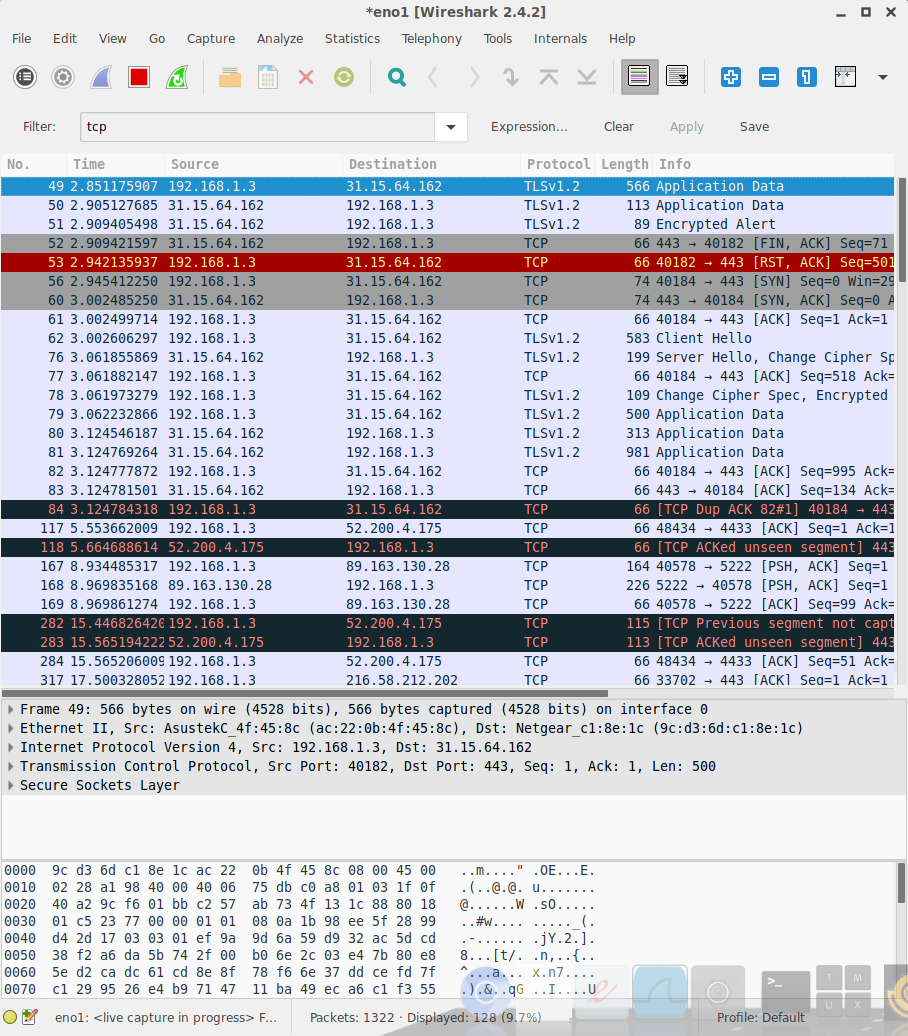
\includegraphics[scale=0.2]{wireshark}
\end{minipage}
\end{frame}
\end{document}